\documentclass[11pt]{article}
\usepackage{graphicx}

\begin{document}
\title{Homework 17}
\author{Colt Bradley}
\date{}
\maketitle
\section{Exercise 1}

For the first exercise, the data is linear. This means we can use the derivation provided in the text. Assigning the elements of the matrices is a simple matter of looping over each element of the imported data. Then we use linear algebra to solve, which yields values of $10.8 m/s$ for g, an error of $2.9\%$.

\begin{figure}[ht]
\centering
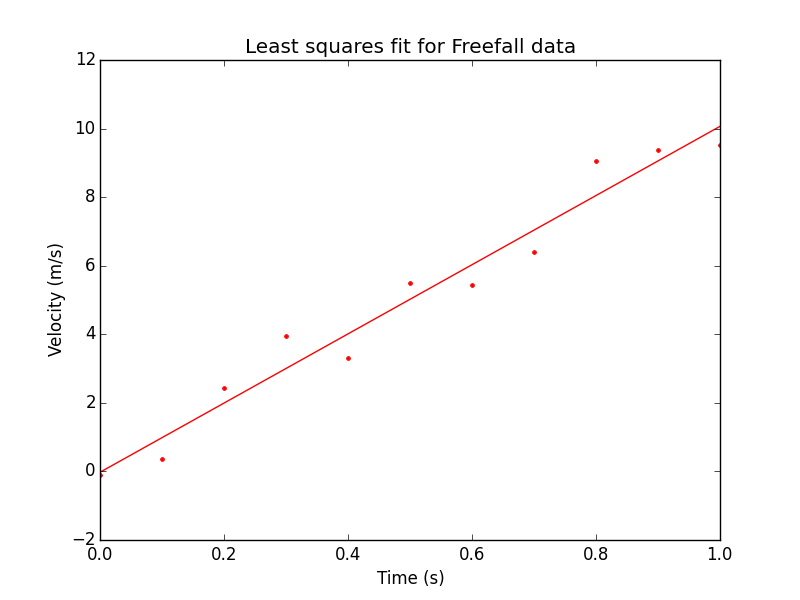
\includegraphics[scale=.5]{freefall.png}
\end{figure}

\section{Exercise 2}

In the second exericse, we use a function from the module ``scipy'' called curve fit. We have data from a sine curve, import it, and run it through this function to determine the amplitude ($2.38$), frequency ($1.43$), and phase($0.52$). 

\begin{figure}[ht]
\centering
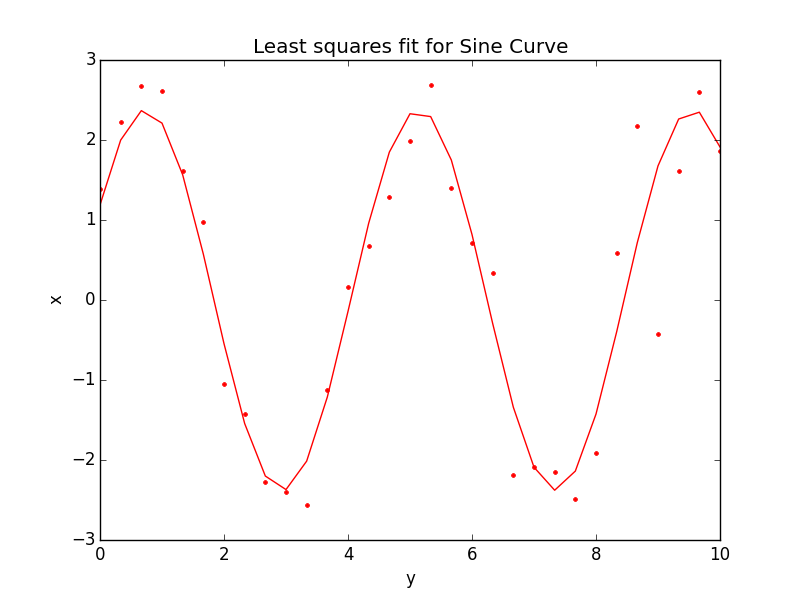
\includegraphics[scale=.5]{sincurve.png}
\end{figure}

\section{Code}
\begin{verbatim}
#Colt Bradley
#3.22.2016
#Lesson 17

import os
os.chdir("C:/Users/Colt/OneDrive/Documents/Professional/School/16spring/PY_251/Lesson 17")

#############################################################################
#functions and modules
#############################################################################

#import modules
import numpy as n
import pylab as p
from scipy.optimize import curve_fit

#relative error calculating function
def error(val, expval):
    return abs(val-expval)/expval

#############################################################################
#Exercise 1
#############################################################################
#import list of data
X, Y = n.loadtxt("freefall.data", usecols = (0, 1), unpack = True)

#define values in matrix. Note that a12, a21 are the same. 
a11 = 0
for i in X:
    a11 += i**2

#sum of all x values
a12 = 0
for i in X:
    a12 += i
a21 = a12
    
#number of elements
a22 = len(X)

#sum of x,y values multipied
r1 = 0
for i,k in zip(X,Y):
    r1 += i*k

#sum of all y values
r2 = 0
for i in Y:
    r2 += i

#use linear algebra to solve the system    
A = n.matrix([[a11,a12],[a21,a22]])
r = n.matrix([[r1],[r2]])
soln = n.linalg.solve(A,r)
a = soln[0,0]
b = soln[1,0]

func = []
for j in X:
    ans = j*a+b
    func.append(ans)

#plot values on the graph
p.close()
p.plot(X,Y,"r.")
p.plot(X,func,"r")
p.title("Least squares fit for Freefall data")
p.xlabel("Time (s)")
p.ylabel("Velocity (m/s)")
p.savefig("freefall.png")
p.show()

print "Exercise 1: \nCalculated g: {:.2f} m/s\nPercent Error: {:.1f}%\n"\
.format(a,error(a,9.8)*100)

#############################################################################
#Exercise 2
#############################################################################
def func(x,a,b,c):
    return a*n.sin(b*x+c)

Xd, Yd = n.loadtxt("sincurvedata.data", usecols = (0, 1), unpack = True)
par, con = curve_fit(func,Xd,Yd)

sin=[]
for i in Xd:
    y = func(i,par[0],par[1],par[2])
    sin.append(y)

p.close()
p.plot(Xd,Yd,"r.")
p.plot(Xd,sin,"r")
p.title("Least squares fit for Sine Curve")
p.xlabel("y")
p.ylabel("x")
p.savefig("sincurve.png")
p.show()
print "Exercise 2:\nAmplitute: {:.3f}\nFrequency: {:.3f}\nPhase: {:.3f}"\
.format(par[0],par[1],par[2])
\end{verbatim}



\end{document}